\documentclass[10pt,a4paper]{article}
\usepackage[utf8]{inputenc}
\usepackage[english]{babel}
\usepackage{amsmath}
\usepackage{amsfonts}
\usepackage{amssymb}
\usepackage{graphicx}
\graphicspath{{figs/}{./}{feynman/build/}}
\begin{document}

\begin{figure}
\centering
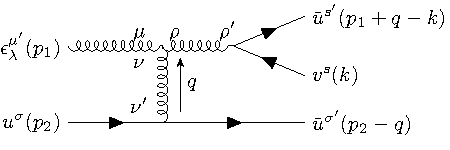
\includegraphics[width=.5\textwidth]{Large-Q-g2qqbar-A.pdf}\\
\vspace{1em}
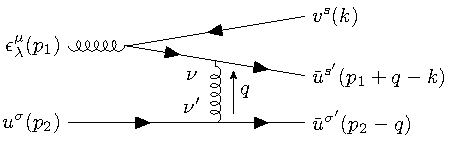
\includegraphics[width=.49\textwidth]{Large-Q-g2qqbar-B.pdf}\hfill
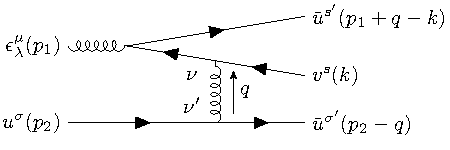
\includegraphics[width=.49\textwidth]{Large-Q-g2qqbar-C.pdf}
\caption{Three diagrams $A$ (Top), $B$ (Bottom left), $C$ (Bottom right) that contribute to the large angle scattering induced gluon splitting into quark-anti-quark pair.}
\end{figure}


\begin{eqnarray}
p_1 &=& (\sqrt{s}, 0, \vec{0})\\
p_2 &=& (0, \sqrt{s}, \vec{0})\\
k &=& (x\sqrt{s}, \frac{k_\perp^2}{x\sqrt{s}}, \vec{k}_\perp)\\
q &\sim& (-\frac{q_\perp^2}{\sqrt{s}}, \frac{q_\perp^2 + k_\perp^2/x - 2\vec{q}_\perp \cdot \vec{k}_\perp}{(1-x)\sqrt{s}}, \vec{k}_\perp)\\
n &=& (0, 1, 0)\\
\epsilon(p) &\sim& (0, \frac{2\vec{\epsilon}_\perp\cdot\vec{p}_\perp}{p^+}, \vec{\epsilon}_\perp)
\end{eqnarray}

The first diagram:
\begin{eqnarray}
i M_A &=& (-ig)^2(-g)f^{abc}(t^b)_{j'j}(t^c)_{i'i} \epsilon_\lambda^\mu(p_1) \\\nonumber
&&\frac{-i}{(p_1+q)^2}\left(g^{\rho\rho'}-\frac{n^{\rho}(p_1+q)^{\rho'}+n^{\rho'}(p_1+q)^\rho}{n\cdot (p_1+q)}\right) \bar{u}^s(p_1+q-k)\gamma_{\rho'}v^{s'}(k) \\ \nonumber
&&\frac{-i}{q^2}\left(g^{\nu\nu'}-\frac{n^{\nu}q^{\nu'}+n^{\nu'}q^\nu}{n\cdot q}\right) \bar{u}^{\sigma}(p_4)\gamma_{\nu'}u^{\sigma'}(p_2) \\ \nonumber
&& \left[g_{\mu\nu}(p_1-q)_\rho + g_{\nu\rho}(2q+p_1)_\rho + g_{\rho\mu}(-2p_1 -q)_\nu \right]\\
&\approx& -g^3 f^{abc}(t^b)_{j'j}(t^c)_{i'i} \delta^{\sigma\sigma'} \epsilon^\mu(p_1) \\\nonumber
&&\frac{1}{(p_1+q)^2} \sum_{\lambda'=\pm}\epsilon_{\lambda'}^{\rho}(p_1+q)\underbrace{\epsilon_{\lambda'}^{*,\rho'}(p_1+q) \bar{u}^s(p_1+q-k)\gamma_{\rho'}v^{s'}(k)}_{iP_{A,\lambda'}^{ss'}} \\ \nonumber
&&\frac{1}{q_\perp^2}\left(g^{\nu\nu'}-\frac{n^{\nu}q^{\nu'}+n^{\nu'}q^\nu}{n\cdot q}\right) (2p_2-q)_{\nu'} \\ \nonumber
&& \left[g_{\mu\nu}(p_1-q)_\rho + g_{\nu\rho}(2q+p_1)_\rho + g_{\rho\mu}(-2p_1 -q)_\nu \right] \\
&=& -g^3 f^{abc}(t^b)_{j'j}(t^c)_{i'i} \frac{1}{(p_1+q)^2}\frac{1}{q_\perp^2} \sum_{\lambda'=\pm}iP_{A,\lambda}^{ss'} \delta^{\sigma\sigma'}  \\ \nonumber
&& \epsilon_\lambda^\mu(p_1)2p_2^{\nu} \epsilon_{\lambda'}^{\rho}(p_1+q) \left[g_{\mu\nu}(p_1-q)_\rho + g_{\nu\rho}(2q+p_1)_\rho + g_{\rho\mu}(-2p_1 -q)_\nu \right]\\
&\approx& -g^3 f^{abc}(t^b)_{j'j}(t^c)_{i'i}\delta^{\sigma\sigma'}\frac{2s}{q_\perp^2} \frac{x(1-x)}{(\vec{k}_\perp-x \vec{q}_\perp)^2} iP_{A,\lambda}^{ss'} 
\end{eqnarray}
The second and third diagram,
\begin{eqnarray}
i M_B &=& i g^3 (t^b t^a)){i'i} t^b{j'j} \delta^{\sigma\sigma'} \frac{2s}{q_\perp^2} \frac{x(1-x)}{k_\perp^2}  iP_{B,\lambda}^{ss'} \\
i M_C &=& -i g^3 (t^a t^b)){i'i} t^b{j'j} \delta^{\sigma\sigma'} \frac{2s}{q_\perp^2} \frac{x(1-x)}{(\vec{k}_\perp-\vec{q}_\perp)^2}  iP_{C,\lambda}^{ss'} 
\end{eqnarray}
The sum of all three diagrams, applying $f^{abc}t^c = -i[t^a, t^b]$
\begin{eqnarray}
i (M_A+M_B+M_C) &=& ig^3 \frac{2s}{q_\perp^2} (t^b)_{j'j} x(1-x)\\\nonumber
&&\left\{(t^a t^b)_{i'i} \left(\frac{iP_{A,\lambda}^{ss'} }{(\vec{k}_\perp-x \vec{q}_\perp)^2} - \frac{iP_{C,\lambda}^{ss'}}{(\vec{k}_\perp-\vec{q}_\perp)^2}\right) -(t^a t^b)_{i'i}\left(\frac{iP_{A,\lambda}^{ss'} }{(\vec{k}_\perp-x \vec{q}_\perp)^2} - \frac{iP_{B,\lambda}^{ss'}}{k_\perp^2}\right) \right\}
\end{eqnarray}


The splitting amplitude:
\begin{eqnarray}
&&\epsilon_{\lambda, \mu} \bar{u}_s(a)\gamma^\mu v_{s'}(b)\\
&=&\frac{1}{\sqrt{2a}\sqrt{2b}}(\xi^T_s a\cdot\sigma, \xi^T_{s} a\cdot \bar{\sigma})
\begin{bmatrix}
\epsilon\cdot\bar{\sigma} & 0 \\
0 & \epsilon\cdot\sigma
\end{bmatrix}
\begin{bmatrix}
b\cdot\sigma \eta_{s'}\\
b\cdot\bar{\sigma} \eta_{s'}
\end{bmatrix}
\\
&=&\frac{1}{2\sqrt{ab}}
\xi_s^T
\begin{bmatrix}
a^- & -a^\perp_L \\
-a^\perp_R & a^+
\end{bmatrix}
\begin{bmatrix}
0 & \sqrt{2}\delta_{\lambda R}\\
\sqrt{2}\delta_{\lambda L} & \frac{\sqrt{2}c^\perp_\lambda}{c^+}
\end{bmatrix}
\begin{bmatrix}
b^- & -b^\perp_L \\
-b^\perp_R & b^-
\end{bmatrix}
\eta_{s'}\\\nonumber
&-&
\frac{1}{2\sqrt{ab}}
\xi_s^T
\begin{bmatrix}
a^+ & a^\perp_L \\
a^\perp_R & a^-
\end{bmatrix}
\begin{bmatrix}
\frac{\sqrt{2}c^\perp_\lambda}{c^+} & -\sqrt{2}\delta_{\lambda R}\\
-\sqrt{2}\delta_{\lambda L} & 0
\end{bmatrix}
\begin{bmatrix}
b^+ & b^\perp_L \\
b^\perp_R & b^-
\end{bmatrix}
\eta_{s'}
\\
&=&\frac{1}{\sqrt{2ab}}
\xi_s^T
\begin{bmatrix}
-a^\perp_L b^- \delta_{\lambda L} - a^- b^\perp_L \delta_{\lambda R} + a^\perp_L b^\perp_R\frac{c^\perp_\lambda}{c^+} &
-a^\perp_L b^\perp_L \delta_{\lambda L} + a^- b^+ \delta_{\lambda R} + a^\perp_L b^+\frac{c^\perp_\lambda}{c^+}
\\
a^+ b^- \delta_{\lambda L} + a^\perp_R b^\perp_R \delta_{\lambda R} - a^+ b^\perp_R\frac{c^\perp_\lambda}{c^+} &
-a^+ b^\perp_L \delta_{\lambda L} - a^\perp_R b^+ \delta_{\lambda R} + a^+ b^+\frac{c^\perp_\lambda}{c^+}
\end{bmatrix}
\eta_{s'}\\\nonumber
&-&\frac{1}{\sqrt{2ab}}
\xi_s^T
\begin{bmatrix}
-a^\perp_L b^+ \delta_{\lambda L} - a^+ b^\perp_R \delta_{\lambda R} + a^+ b^+\frac{c^\perp_\lambda}{c^+} &
-a^\perp_L b^\perp_L \delta_{\lambda L} - a^+ b^- \delta_{\lambda R} + a^+ b^\perp_L\frac{c^\perp_\lambda}{c^+}
\\
-a^- b^+ \delta_{\lambda L} - a^\perp_R b^\perp_R \delta_{\lambda R} + a^\perp_+ b^+\frac{c^\perp_\lambda}{c^+} &
-a^- b^\perp_L \delta_{\lambda L} - a^\perp_R b^- \delta_{\lambda R} + a^\perp_R b^\perp_L\frac{c^\perp_\lambda}{c^+}
\end{bmatrix}
\eta_{s'}
\end{eqnarray}
Dropping terms that is of order $(+)(-)$ or $(\perp)(\perp)$ or $(\perp)(-)$,
\begin{eqnarray}
&&\epsilon_{\lambda, \mu} \bar{u}_s(a)\gamma^\mu v_{s'}(b)\\
&=& \frac{1}{\sqrt{2ab}}
\xi_s^T
\begin{bmatrix}
a^\perp_L b^+ \delta_{\lambda L} + a^+ b^\perp_R \delta_{\lambda R} - a^+ b^+\frac{c^\perp_\lambda}{c^+} & 0\\
0 & -a^+ b^\perp_L \delta_{\lambda L} - a^+ b^\perp_R \delta_{\lambda R} + a^+ b^+\frac{c^\perp_\lambda}{c^+}
\end{bmatrix}
\eta_{s'}
\end{eqnarray}
The module square of one splitting amplitude, sum over spins and average over polarization is ($a^+ = xc^+, b^+ = (1-x)c^+$ and $c = a+b$),
\begin{eqnarray}
\frac{1}{2}\sum_\pm |P|^2 = \frac{2(x^2 + (1-x)^2)}{x(1-x)} \left((1-x)\vec{a}_\perp-x\vec{b}_\perp\right)^2.
\end{eqnarray}
This result goes back to the standard splitting function if it is computed in the frame where $a_\perp = -b_\perp$. 
However, there is no such frame that $a_\perp = -b_\perp$ satisfies simultaneously for the splitting in diagram A, B and C, therefore the result gets complicated,
\begin{eqnarray}
\frac{1}{2d_F 2d_A}\sum_{\lambda, s, s', \sigma, \sigma', a, b}|M^2|_{g+q\rightarrow q+\bar{q}+q} &=& g^6 \frac{2C_F}{d_A}\frac{4s^2}{q_\perp^4}x(1-x)\overbrace{\frac{(x^2+(1-x)^2)}{2}}^{P(x)}  \\\nonumber
&\times&\left(C_F \vec{A}^2 + C_F \vec{B}^2 - (2C_F- C_A)\vec{A}\cdot\vec{B}\right)
\end{eqnarray}
Where the $\vec{A}$ and $\vec{B}$ is,
\begin{eqnarray}
\vec{A} &=& \frac{\vec{k}_\perp - x\vec{q}_\perp}{(\vec{k}_\perp - x\vec{q}_\perp)^2} -  \frac{\vec{k}_\perp - \vec{q}_\perp}{(\vec{k}_\perp - \vec{q}_\perp)^2} \\
\vec{B} &=& \frac{\vec{k}_\perp - x\vec{q}_\perp}{(\vec{k}_\perp - x\vec{q}_\perp)^2} -  \frac{\vec{k}_\perp}{\vec{k}_\perp^2}
\end{eqnarray}

Similarly for $g+q\rightarrow g+g+q$, and $q+q\rightarrow q+g+q$
\begin{eqnarray}
\overline{|M^2|}_{g+q\rightarrow g+g+q} &=& g^6 \frac{C_A}{d_F}\frac{4s^2}{q_\perp^4}x(1-x) ]\overbrace{C_A\frac{1+x^4+(1-x)^4}{x(1-x)}}^{P(x)}   \\\nonumber
&\times&\left(\vec{A}^2 + \vec{B}^2 - \vec{A}\cdot\vec{B}\right)\\
\vec{A} &=& \frac{\vec{k}_\perp - x\vec{q}_\perp}{(\vec{k}_\perp - x\vec{q}_\perp)^2} -  \frac{\vec{k}_\perp - \vec{q}_\perp}{(\vec{k}_\perp - \vec{q}_\perp)^2} \\
\vec{B} &=& \frac{\vec{k}_\perp - x\vec{q}_\perp}{(\vec{k}_\perp - x\vec{q}_\perp)^2} -  \frac{\vec{k}_\perp}{\vec{k}_\perp^2}
\end{eqnarray}

and

\begin{eqnarray}
\overline{|M^2|}_{g+q\rightarrow g+g+q} &=& g^6 \frac{C_F}{d_F}\frac{4s^2}{q_\perp^4}x(1-x) \overbrace{C_F\frac{1+(1-x)^2}{x}}^{P(x)}  \\\nonumber
&\times&\left(\vec{A}^2 + \vec{B}^2 - \left(2-\frac{C_A}{C_F}\right)\vec{A}\cdot\vec{B}\right)\\
\vec{A} &=& \frac{\vec{k}_\perp - \vec{q}_\perp}{(\vec{k}_\perp - \vec{q}_\perp)^2} -  \frac{\vec{k}_\perp - x\vec{q}_\perp}{(\vec{k}_\perp - x\vec{q}_\perp)^2} \\
\vec{B} &=& \frac{\vec{k}_\perp - \vec{q}_\perp}{(\vec{k}_\perp - \vec{q}_\perp)^2} -  \frac{\vec{k}_\perp}{\vec{k}_\perp^2}
\end{eqnarray}


\end{document}